Since the UNet embeddings are the most promising for clustering based on input corruptions we will proceed with this approach. Apart from dimensionality reduction methods used in section \ref{section:unet-embeddings-dim-reduction}, PaCMAP clustering was applied. Its detailed description can be found in section \ref{section:pacmap}. 
\begin{figure}[htb]
	\begin{center}
		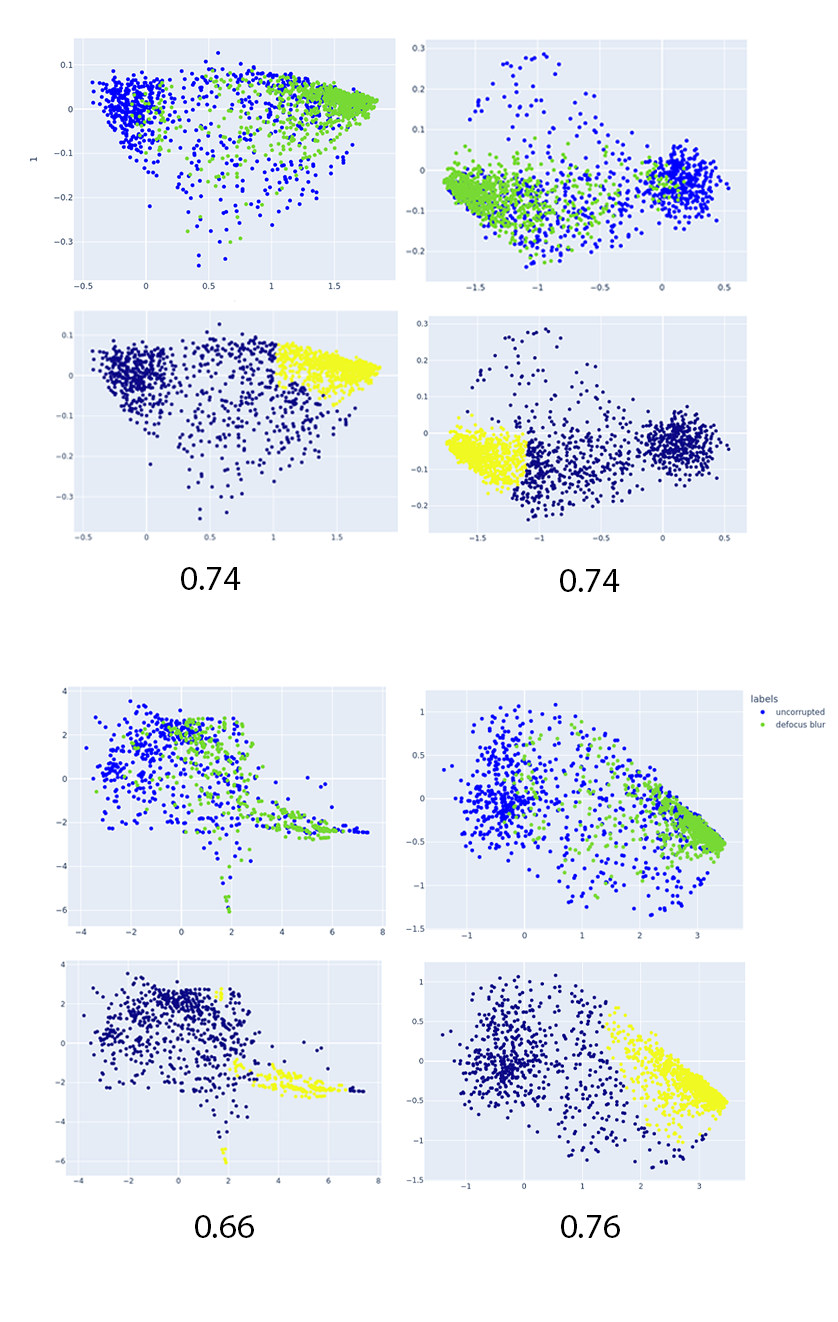
\includegraphics[width=\linewidth]{bilder/unet-embeddings/PacMAP.png}
		\caption{Clustering of UNet embeddings after PacMAP}
		\label{fig:unet-clustering}
	\end{center}
\end{figure}

PaCMAP allows a more flexible hyperparameter tuning in order to preserve local and global relations from high-dimensional data and as a result a better clustering can be found. As usual PaCMAP was trained using "good" training data only, meaning no corruptions were introduced. And only when the transformation from high-dimensional into a lower-dimensional space was found, corrupted crops were projected using this transformation. Figure \ref{fig:unet-clustering} presents results of training PaCMAP with four different hyperparametrization settings. There are three hyperparameters that were changed here: \textit{MN\_ratio}, \textit{FP\_ratio} and \textit{n\_neighbors}. A detailed explanation of their influence was also given in Section \ref{section:pacmap}. From left to right in Figure \ref{fig:unet-clustering} the hyperparameters were taken from Table \ref{table:pacmap-hyperparametrization}:

\begin{table}
	\centering
	\begin{tabularx}{\linewidth}{|ccc|}
		\hline
		\textit{MN\_ratio}
		&\textit{FP\_ratio}
		&\textit{n\_neighbors}
		\\\hline\hline
		$0.5$ & $0.1$ & $10$ \\\hline
		$0.1$ & $0.1$ & $10$\\\hline
		$0.5$ & $0.5$ & $2$\\\hline
		$0.1$ & $0.5$ & $10$\\\hline
	\end{tabularx}
	\caption[PaCMAP hyperparameters]%
	{PaCMAP hyperparameters}
	\label{table:pacmap-hyperparametrization}
\end{table}

In this case a cluster of green dots represents the projected UNet embeddings of images corrupted with defocus blur with severity level $4$, which is already a strong corruption and leads to unacceptable predictions of the model, that did not have defocus blur augmentations. However, these points are still strongly mixed with non-corrupted ones. In order to check how separable they are unsupervised clustering DBSCAN algorithm was used. Results of this clustering are shown in Figure \ref{fig:unet-clustering-sev-levels}. The density based clustering approach utilized here was described in more details in section \ref{section:dbscan}. 

\begin{figure}[htb]
	\begin{center}
		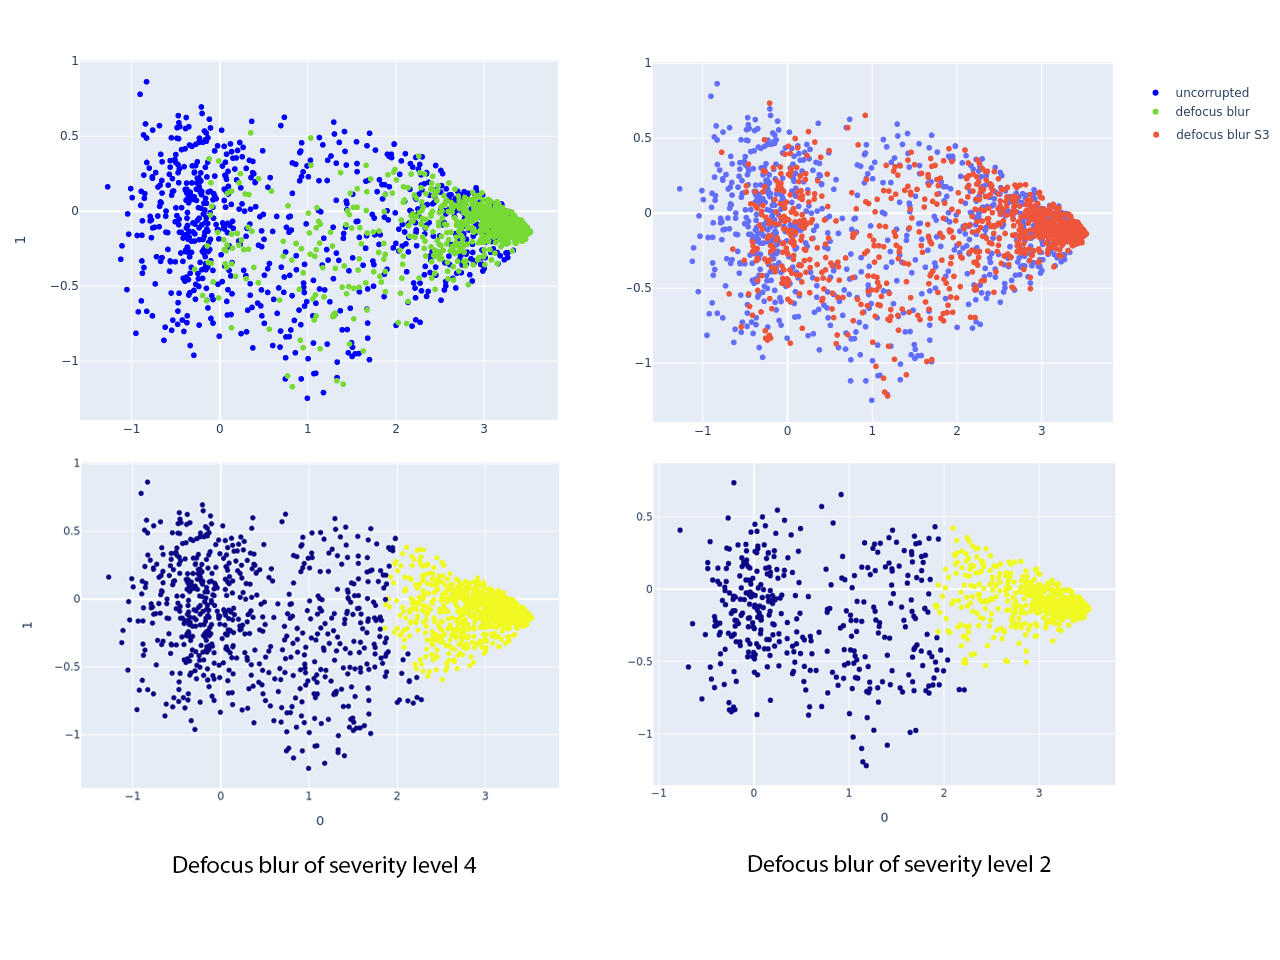
\includegraphics[width=0.6\linewidth]{bilder/unet-embeddings/db-levels.png}
		\caption{Clustering of UNet embeddings after PacMAP for different severities levels}
		\label{fig:unet-clustering-sev-levels}
	\end{center}
\end{figure}

After training DBSCAN on non-corrupted crops embeddings it has recognized a class on the right (yellow dots) as a cluster and the rest of the points (blue ones) as noise, because they have quite low density in comparison to the yellow cluster. This is not a problem if we consider noisy points simply as a separate cluster. For such clustering defocus blur of level $4$ splits the crops between two clusters with an F1-score of $0.74$. In Figure \ref{fig:unet-clustering-sev-levels} on the right red points represent projection of image embeddings after corrupting them with a defocus blur of severity level $3$. In this case they are mixed with non-corrupted projections even stronger. Here prediction of already trained DBSCAN drops to F1-score of $0.64$.

Overall UNet embeddings do express clustering of corrupted embeddings to a small extent, however not strongly enough to use it in practice. Here the autoencoder would be a more suitable approach, however brightness normalization has to take place first. It is recommended to further drive research here in the direction of contrastive learning algorithms, specifically following the approach proposed by \cite{csi}.